\documentclass{journal}
\usepackage{graphicx}	% package for using graphics
\usepackage{float}	% package for positioning figures

\title{AIRFRAME DESIGN FINAL REPORT}

\author{Nathan Pettit}


\begin{document}
	
	\maketitle	
	\section{Introduction}
	This report covers all the work and research done for the ME EN 497R Airframe Design track.
	It is a compilation of projects 1, 2 and 3 of this track. This final report is broken up into 3 parts: airfoil analysis, wing and tail analysis, and wing and tail design.\\
	
	\section{Airfoil Analysis}
	This section reviews research done on airfoils. There are 5 areas that are covered in this research. One, it explores the effect of airfoil angle of attack on lift, drag, and moment. Two, it compares data collected by Xfoil to experimental data. Three, it explores the effect of different Reynold's numbers on airfoil polar. Four, it explores the effect of different airfoil thicknesses. And five, it explores the effect of different airfoil cambers.\\
	
	The results of this research came from evaluating airfoils using the Xfoil library in Julia, as well as writing new functions to help in evaluating the airfoils. There were 4 functions that were  used:\\
	
	\begin{enumerate}
		\item alter\_thicknesscamber() - this evaluated airfoils of varying thicknesses and cambers and plotted their lifts and drags together in order to compare them
		\item get\_coefficients() - this was a helper function that was used to calculate the coefficients of lift, drag, and moment and return them to other functions that needed those calculations done
		\item alter\_reynolds() - this evaluated an airfoil using varying Reynolds numbers and plotted their lift, drag, and moment in order to compare them
		\item auto\_sweep() - this calculated and plotted an airfoil's lift, drag, and moment with varying airfoil angles of attack
	\end{enumerate}
	
	\subsection{Airfoil Angle  of Attack}
	One of the most stressed parts of this research was seeing how different airfoil angles of attack affected the lift, drag, and moment on the airfoil. In order to see those relationships, only the coefficients of drag, lift, and moment needed to evaluated, rather than the moment and the forces of lift and drag. This is because in calculating lift, drag, and moment, the only parts that differ are the coefficients. Figure \ref{fig:aoa-coefficients} shows the relationships between lift, drag, and moment and \(\alpha\) for a NACA 2412 airfoil.\\
	
	\begin{figure}[H]
		\centering
		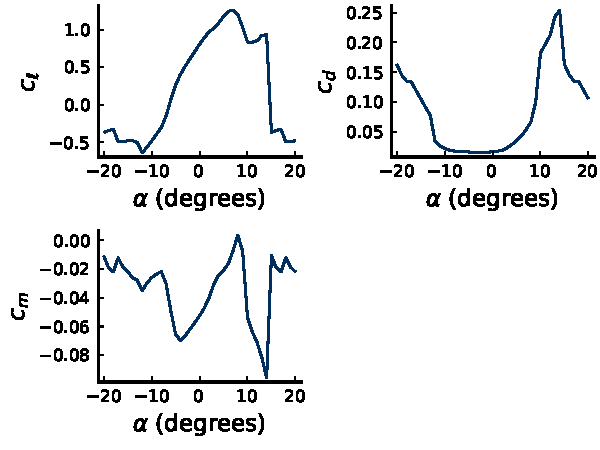
\includegraphics{../graphics/aoa-coefficients.pdf}
		\caption{\emph{This figure shows coefficients of lift, drag, and moment plotted against angle of attack for a NACA 2412 airfoil.}}
		\label{fig:aoa-coefficients}
	\end{figure}
	
	The coefficients of lift (\(c_\ell\)) and drag (\(c_d\)) both increase as angle of attack (\(\alpha\)) increases, because as the angle increases, the pressure differential between the top and bottom of the airfoil becomes larger. This also increases coefficient of moment (\(c_m\)). It is also important to note that figure \ref{fig:aoa-coefficients} establishes that lift is negative when \(\alpha\) is less than zero, which makes sense, and that the zero-lift angle of attack is somewhere between 0 and 0.5 degrees.It appears that stall takes place at an angle of attack of about 10 degrees. This can be cleary seen on the lift and drag plots.\\
	
	\subsection{Airfoil Polar Comparison}
	The results gained from Xfoil were plotted against experimental data from a study done on the NACA 2412 airfoil (see figure \ref{fig:airfoil-comparison}).\\
	
	\begin{figure}[H]
		\centering
		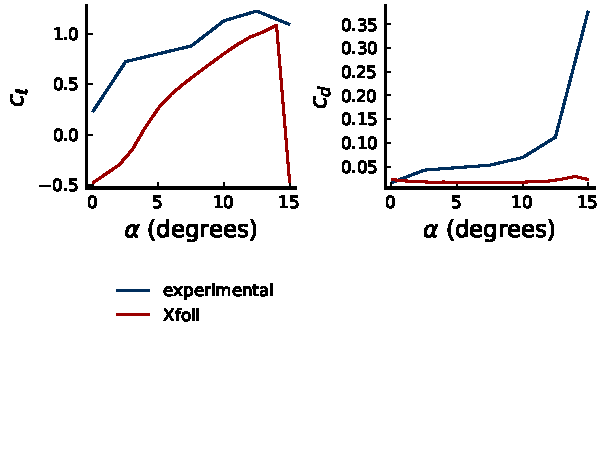
\includegraphics{../graphics/airfoil-compare.pdf}
		\caption{\emph{This figure compares data collected experimentally to data collected from Xfoil.}}
		\label{fig:airfoil-comparison}
	\end{figure}
	
	It is interesting to see that the experimental lift curve looks very similar to the one obtained from Xfoil, expect shifted up. Also, the drag curves between experimental and Xfoil are very different. The reason for this is unknown, although it might be an error in Xfoil calculations.\\
	
	\subsection{Effect of Reynold's Number}
	The Reynold's number is an indicator of how viscous the fluid that an airfoil is traveling through is. A high Reynold's number is an indicator that fluid flow will be turbulent, where as a low Reynold's number is an indicator of laminar flow. In figure \ref{fig:altered-reynolds}, the relationships between Reynold's number and the coefficients are shown.\\
	
	\begin{figure}[H]
		\centering
		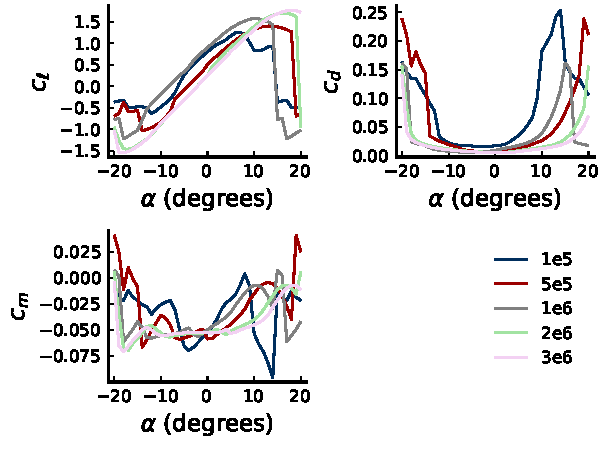
\includegraphics{../graphics/altered-reynolds.pdf}
		\caption{\emph{This figure shows plots of lift, drag, and moment for varying Reynold's numbers.}}
		\label{fig:altered-reynolds}
	\end{figure}
	
	As the Reynold's number increases, the lift curves become more steep. However, it is the opposite with drag and moment. As the Reynold's number increases, the curves of drag and moment become more leveled out. These results make logical sense, because whether with turbulent or laminar flow, lift generally is not affected significantly across varying angles of attack. On the other hand, higher Reynold's numbers and therefore more turbulent flow decreases the drag and moment at more extreme angles of attack (see figure \ref{fig:altered-reynolds}).\\
	
	\subsection{Effect of Airfoil Thickness and Camber}
	The thickness of an airfoil is the greatest distance between the upper and the lower surfaces of an airfoil. In figure \ref{fig:altered-thickness}, the relationship between airfoil thickness and the coefficients of lift, drag, and moment can be seen.\\
	
	\begin{figure}[H]
		\centering
		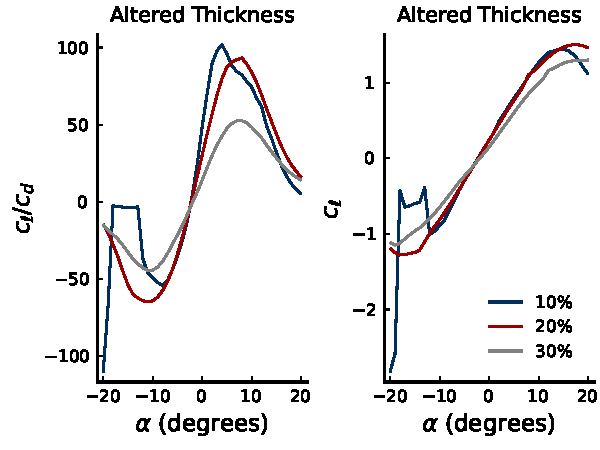
\includegraphics{../graphics/altered-thickness.pdf}
		\caption{\emph{This figure shows the plots of ratio of lift to drag coefficients and coefficient of lift.}}
		\label{fig:altered-thickness}
	\end{figure}
	
	As the thickness of the airfoil increases, the ratio of lift to drag curve becomes more shallow. This is because increasing thickness leads to lift and drag becoming closer and closer to each other. It is interesting to see though that no matter the thickness, the zero lift angle of attack remains the same (see figure \ref{fig:altered-thickness}).\\
	
	The camber of an airfoil is the asymmetry between the two acting surfaces of an airfoil. An airfoil with zero camber is symmetric. In figure \ref{fig:altered-camber}, the effect of different cambers can be seen.\\
	
	\begin{figure}[H]
		\centering
		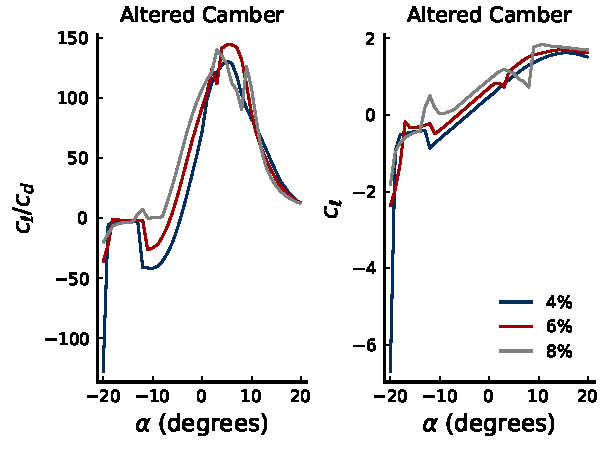
\includegraphics{../graphics/altered-camber.pdf}
		\caption{\emph{This figure shows the plots of ratio of lift to drag coefficients and coefficient of lift.}}
		\label{fig:altered-camber}
	\end{figure}
	
	As the camber of the airfoil increases, the lift to drag ratio becomes higher and the whole curve is shifted upwards. This also happened with the coefficient of lift. This also means that the zero lift angle of attack became greater with increasing camber.\\
	
	\section{Airframe Analysis}
	
	This section covers research done on airframes using the VortexLattice.jl library, specifically how aspect ratio and efficiency are related, how tail volume ratios affect stability derivatives, and how angle of attack affects the lift coefficient.\\
	
	The results of this research came from evaluating airframes using VortexLattice.jl, as well as writing new functions to help in evaluating the airframes. There were 4 functions that were  used:
	
	\begin{enumerate}
		\item aoa\_effect() - this evaluated airframes and calculated their coefficient of lift for varying angles of attack 
		\item wing\_efficiency() - this calculated the efficiency of airframes with varying aspect ratios; it did this by calculating the lift and drag coefficients for every aspect ratio
		\item stability\_derivatives() - this calculated the stability derivatives for airframes with different horizontal and vertical tail ratios
		\item vortex\_lattice() - this was the main function that performed all the necessary VortexLattice calculations for the other functions 
	\end{enumerate}

	\subsection{Aspect Ratio vs. Efficiency}
	
	In order to see the relationship between aspect ratio and the efficiency, the wing\_efficiency() function was used. When it was run, it calculated the inviscid span efficiency (see equation \ref{eqn:efficiency}) for airframes with aspect ratios (see equation \ref{eqn:aspect-ratio}) ranging from 3 to 15.\\
	
	\begin{equation}
		e_{inv} = \frac{C_L^2}{\pi{ARC_D}}
		\label{eqn:efficiency}
	\end{equation}
	
	\begin{equation}
		AR = \frac{b}{c} = \frac{b^2}{S_{ref}}
		\label{eqn:aspect-ratio}
	\end{equation}
	
	After the program calculated the efficiency, it produced a plot shown in figure \ref{fig:efficiency}.\\
	
	\begin{figure}[H]
		\centering
		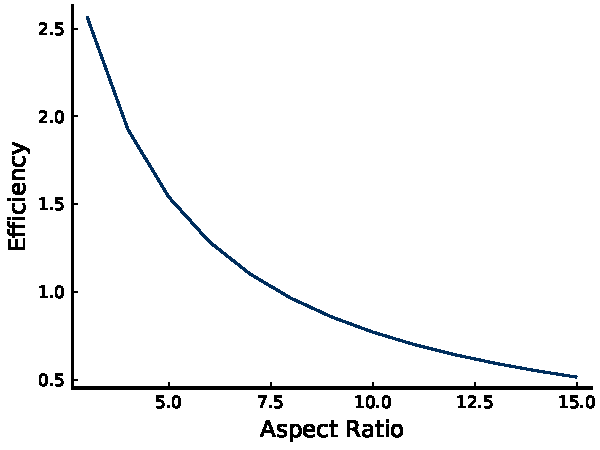
\includegraphics{../graphics/efficiency.pdf}
		\caption{\emph{This diagram shows the relationship between aspect ratio and inviscid span efficiency.}}
		\label{fig:efficiency}
	\end{figure}
	
	In reality, there is actually no physical relationship between an airframe's aspect ratio and its efficiency, but figure \ref{fig:efficiency} does mathematically plot it correctly. However, that plot is simply the definition of inviscid span efficiency.\\
	
	\subsection{Tail Volume Ratios vs Stability Derivatives}
	
	Another characteristic of these airframes that was observed was their stability derivatives. Stability derivatives were calculated for airframes with different tail volume ratios, both vertical and horizontal. The definitions of those ratios are equations \ref{eqn:vtail-ratio} and \ref{eqn:htail-ratio}. The stability derivatives that are affected by a change in vertical tail volume ratio are \(C_{\ell{b}}\) and \(C_{nb}\). \(C_{\ell{b}}\) is the stability derivative associated with roll stability. \(C_{nb}\) is the stability derivative associated with yaw stability. An airframe is stable if \(C_{\ell{b}}\) is less than 0 and \(C_{nb}\) is greater than 0.\\
	
	\begin{equation}
		V_v = \frac{l_vS_v}{Sb}
		\label{eqn:vtail-ratio}
	\end{equation}
	
	\begin{equation}
		V_h = \frac{l_tS_t}{SC_{ma}}
		\label{eqn:htail-ratio}
	\end{equation}
	
	In figure \ref{fig:vtail-stability} , we can see that the airframe is stable for vertical tail volume ratios greater than 0.003, but it becomes unstable when the ratio is less than 0.003, at around 0.002. The stability derivatives that are affected by a change in horizontal tail volume ratio are \(C_{La}\) and \(C_{ma}\). An airframe is stable if \(C_{La}\) is greater than 0 and \(C_{ma}\) is less than 0. Figure \ref{fig:htail-stability} shows that the airframe is stable for horizontal tail volume ratios greater than 0.05, but becomes unstable when the ratio is less than 0.05, at around 0.025.\\
	
	\begin{figure}[H]
		\centering
		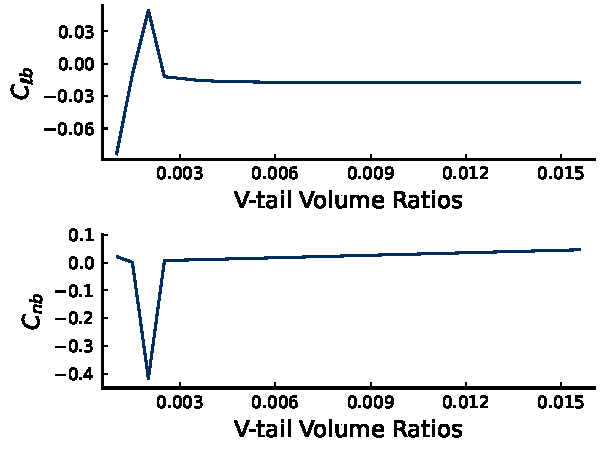
\includegraphics[scale=0.73]{../graphics/vtail-stability.pdf}
		\caption{\emph{This diagram shows the relationship between vertical tail volume ratio, \(C_{\ell{b}}\), and \(C_{nb}\).}}
		\label{fig:vtail-stability}
	\end{figure}
	
	\begin{figure}[H]
		\centering
		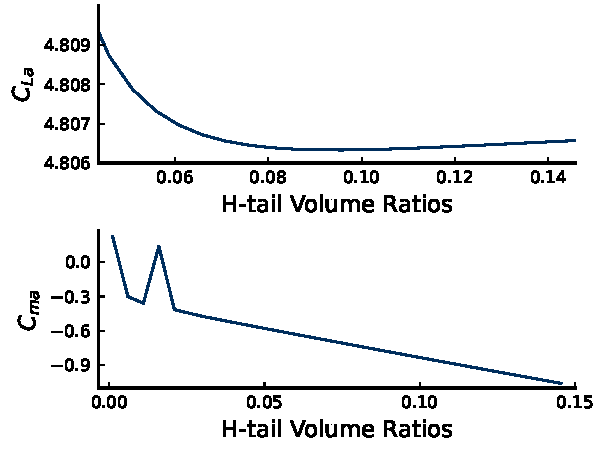
\includegraphics[scale=0.73]{../graphics/htail-stability.pdf}
		\caption{\emph{This diagram shows the relationship between horizontal tail volume ratio, \(C_{La}\), and \(C_{ma}\).}}
		\label{fig:htail-stability}
	\end{figure}
	
	These ratios are arbitrary and will be different among models, but they are still extremely important.\\
	
	\subsection{Angle of attack vs lift coefficient}
	
	In previous research about airfoils, I found that as angle of attack increases, the lift coefficient also increases, up to a certain point. At that point, the lift coefficient sharply drops, and this is where stall takes place. In that previous research, Xfoil.jl was used to calculate the lift coefficient for varying angles of attack. A relationship between angle of attack and lift was also tried to be found here, but instead of using Xfoil.jl, VortexLattice.jl was used. A plot was produced showing the relationship between angle of attack and lift (see figure \ref{fig:aoa-lift}).\\
	
	\begin{figure}[H]
		\centering
		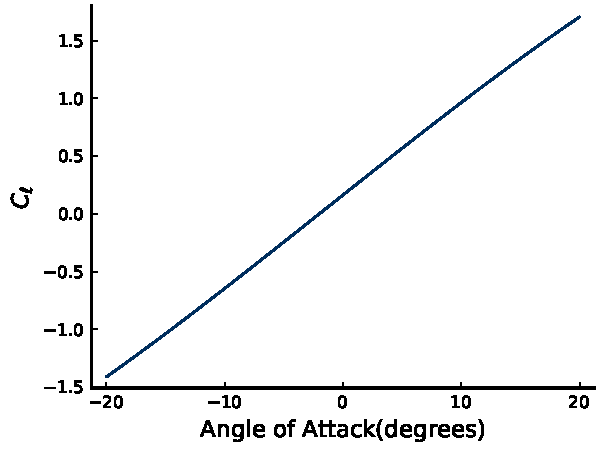
\includegraphics{../graphics/aoa-lift.pdf}
		\caption{\emph{This diagram shows the relationship between angle of attack and lift for an airframe.}}
		\label{fig:aoa-lift}
	\end{figure}
	
	In comparison to the plot created using Xfoil.jl (see figure \ref{fig:aoa-coefficients}), figure \ref{fig:aoa-lift} looks very similar between angles of attack of -10 and 10. However, past those angles of attack is where it differs. In the Xfoil plot, it shows very clearly where stall would take place, but in this VortexLattice plot, the plot continues linearly and never drops off, never indicating stall. This is why the Vortex Lattice method is not always a great choice for investigating airframes. It is only accurate when the angle of attack is small, because it assumes that the flow is inviscid at all angles of attack. This is why in figure \ref{fig:aoa-lift} it looks very linear and doesn't indicate where stall would take place, where as the Xfoil plot does.\\
	
	\section{Airframe Aerodynamic Design}
	
	This report covers the work done in learning how to optimize an airframe with specific parameters, using techniques and knowledge learned previously. The goal was to design an airframe that can lift 0.5 kilograms, has a wingspan no greater than 1.5 meters, and is stable.\\
	
	The results of this research came from evaluating potential airframe solutions using VortexLattice.jl, as well as writing new functions to help in optimizing the airframe design. There were 4 functions that were  used:\\
	
	\begin{enumerate}
		\item optimize\_airframe() - this was the main function that optimized the airframe so that it met the specified requirements and was the most efficient; it employed the use of all the other functions in order to find the optimized airframe
		\item aoa\_coefficients() - this calculated the lift and drag coefficients for a given airframe design for a range of angles of attack.
		\item vortex\_lattice() - this was the function that performed all the necessary VortexLattice calculations for the other functions 
	\end{enumerate}
	
	In order to optimize the airframe, the process, discussed in the introduction to "Engineering Design Optimization" by Joaquim R.R.A. Martins and Andrew Ning, was followed. The objective function  that was minimized was the equation used to calculate the velocity needed to produce the necessary lift to carry 0.5 kilograms (see equation \ref{eqn:needed-velocity}).\\
	
	\begin{equation}
		V = \sqrt{\frac{L}{(0.5)(C_L)(\rho)(S_{ref})}}
		\label{eqn:needed-velocity}
	\end{equation}
	
	\begin{itemize}
		\item \(L\) - the lift needed to takeoff with 0.5 kilograms, in this case 4.905 N
		\item \(\rho\) - the density of the air (1.225 \(kg/m^3\))
		\item \(S_{ref}\) - the reference area, in this case the wing area
	\end{itemize}
	
	The design variables that were altered in order to minimize that function was the mean aerodynamic chord length of the wing and the length from wing to tail on the airframe. The reason I chose these design variables was because I knew that the airframe that would generate the most lift would have the max wingspan possible (so in this case 1.5 m), and so altering the chord length would help me find the wing that needed the least speed to takeoff. I also chose the length from wing to tail as a design variable because I knew altering it would change how stable the airframe was. However, as I worked with these design variables, it was discovered that the greater the length from wing to tail, the more stable the airframe. For this reason, I put an upper limit on that length to be 2.0 m, so that the found airframe would be realistic. I also put a constraint on the aspect ratio of the wing, which was that it had to be greater than 2.0. The way that I found the optimal airframe was I changed those design variables together, so that it found the airframe that took off at the least velocity, but was the most stable. The efficiency of the airframe with different wing taper ratios was also evaluated by plotting the lift coefficient distribution against the optimal distribution, which was a ellipse. The ideal taper ratio was the one that produced a lift coefficient distribution closest to that elliptical distribution. This was done so that the final airframe design not only optimized my objective function, but was also the most efficient design.\\
	
	After running the optimize\_airframe() function, it found that the most optimized airframe was one that had the following characteristics (figure \ref{fig:ideal_design} shows what the design looks like):
	
	\begin{itemize}
		\item span length = 1.5 meters
		\item mean aerodynamic chord length = 0.7222 meters
		\item length from wing to tail = 2.0 meters
		\item taper = 1.0
		\item lift coefficient = 0.04616576328871639
		\item velocity needed to produce necessary lift = 12.653929077220258 m/s
	\end{itemize}
	
	\begin{figure}[H]
		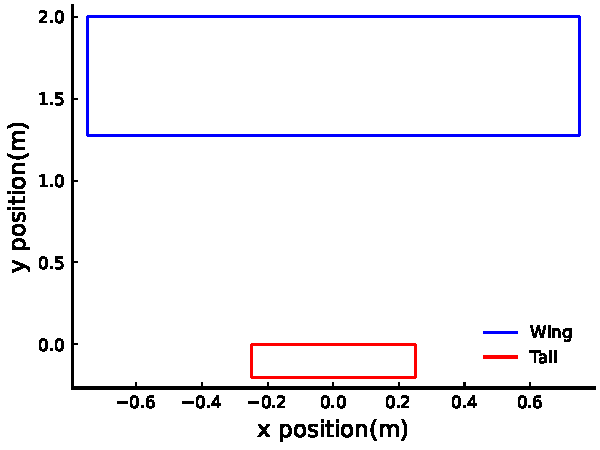
\includegraphics{../graphics/ideal_design.pdf}
		\caption{\emph{This figure shows the design of the optimized airframe.}}
		\label{fig:ideal_design}
	\end{figure}
	
	The aforementioned necessary lift was 4.905 Newtons. This number was found by multiplying 0.5 kilograms by 9.81 \(m/s^2\), which is the acceleration due to gravity. It is also important to note that the optimize\_airframe() function accounts for stability and makes sure that the airframe is the most stable, and so this airframe is the most stable one under the given constraints. In order to show that this airframe has been optimized, other airframes have been evaluated in order to show correctness.\\
	
	\subsection{Altered Mean Chord Length}
	
	When evaluating an airframe that has a mean chord length that is less than 0.7222 m (I used 0.6 m for comparison), it was found that the velocity needed to generate the necessary lift was 13.049496968197154 m/s, which is greater than than the velocity needed for the optimized airframe. This shows that airframes with smaller mean chord lengths are not more optimized, as they need a greater velocity to lift the 0.5 kilograms.\\
	
	\begin{figure}[H]
		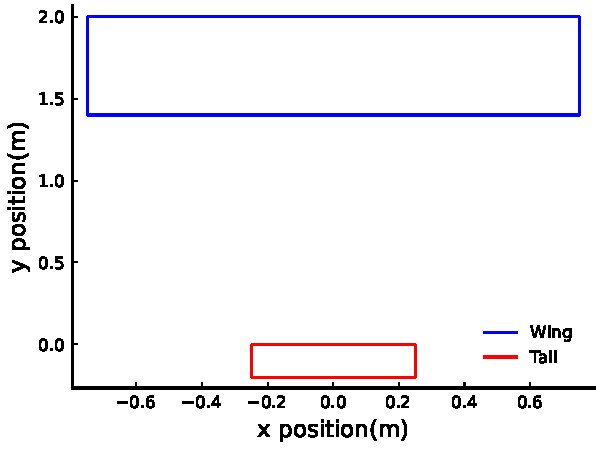
\includegraphics{../graphics/chord_design.pdf}
		\caption{\emph{This figure shows the design of an airframe with a chord length of 0.6 m.}}
		\label{fig:chord_design}
	\end{figure}
	
	An airframe with a greater chord length was not evaluated for comparison, because of the constraint I put on the aspect ratio. 0.7222 m was the largest possible chord length that kept the aspect ratio of the wing greater than 2.0.\\
	
	Plots showing the lift coefficient vs. angle of attack and drag coefficient vs. angle of attack for these 2 designs are given (see figures \ref{fig:chord_cl} and \ref{fig:chord_cd}).
	
	\begin{figure}[H]
		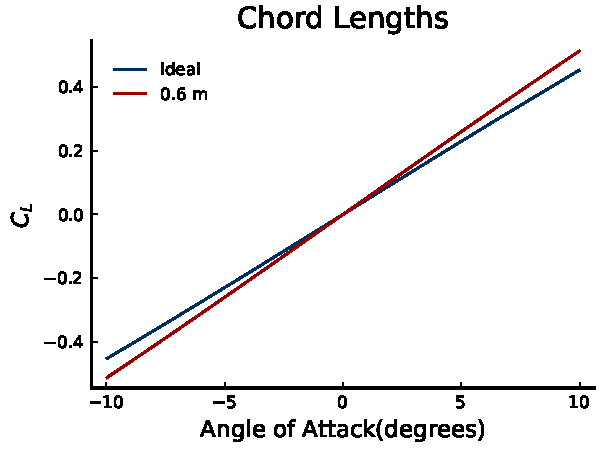
\includegraphics{../graphics/chord_cl.pdf}
		\caption{\emph{This figure shows the lift coefficients for varying angles of attack for the 2 designs evaluated using different mean chord lengths.}}
		\label{fig:chord_cl}
	\end{figure}
	\begin{figure}[H]
		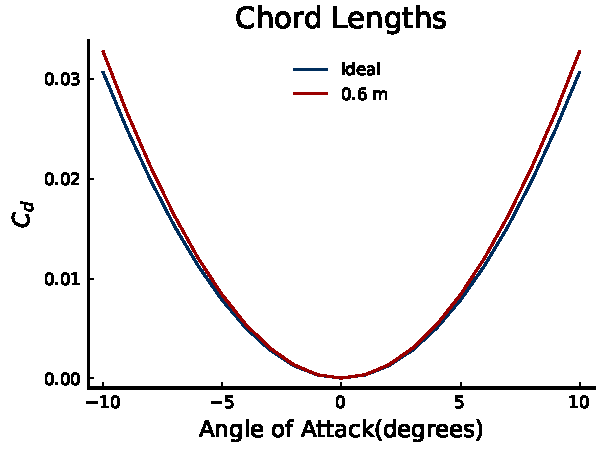
\includegraphics{../graphics/chord_cd.pdf}
		\caption{\emph{This figure shows the drag coefficients for varying angles of attack for the 2 designs evaluated using different mean chord lengths.}}
		\label{fig:chord_cd}
	\end{figure}
	
	\subsection{Altered Length from Wing to Tail}
	
	When evaluating an airframe that has a length from wing to tail that is less than 2.0 m (I used 1.0 m), it was found that the velocity needed to generate the necessary lift doesn't change. However, the airframe is less stable as the yaw stability derivative(\(C_{nb}\)) is less than the yaw stability derivative for the optimized airframe. Therefore, as the length from wing to tail is decreased, the airframe becomes less stable.\\
	
	Figures showing the lift and drag coefficients vs. angle of attack for the 2 designs are given (see figures \ref{fig:wingtail_cl} and \ref{fig:wingtail_cd}). 
	
	\begin{figure}[H]
		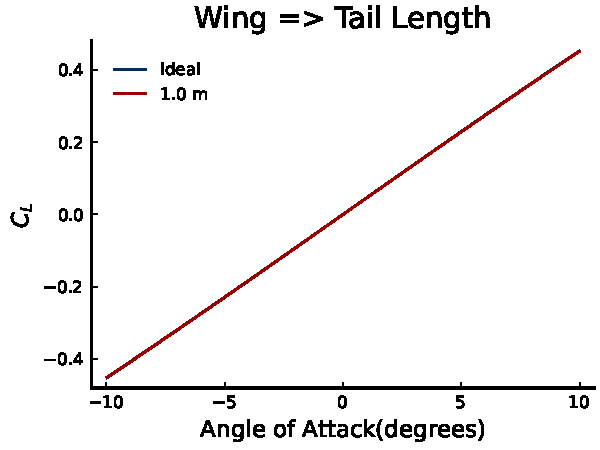
\includegraphics{../graphics/wingtail_cl.pdf}
		\caption{\emph{This figure shows the lift coefficient vs. angle of attack for the 2 designs evaluated.}}
		\label{fig:wingtail_cl}
	\end{figure}
	\begin{figure}[H]
		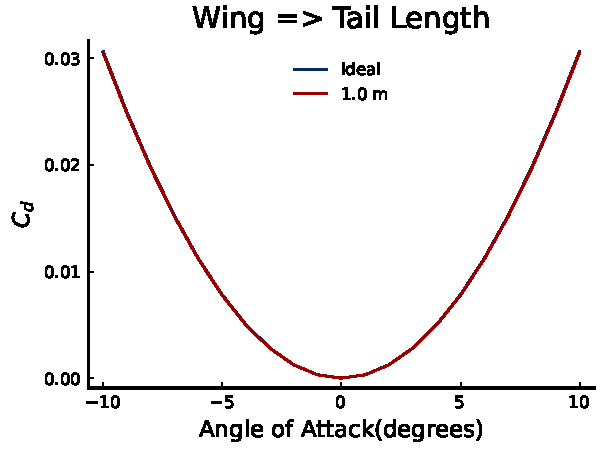
\includegraphics{../graphics/wingtail_cd.pdf}
		\caption{\emph{This figure shows the drag coefficient vs. angle of attack for the 2 designs evaluated.}}
		\label{fig:wingtail_cd}
	\end{figure}
	
	Figure \ref{fig:length_design} shows the design of an airframe with a length from wing to tail of 1.0 m.
	
	\begin{figure}[H]
		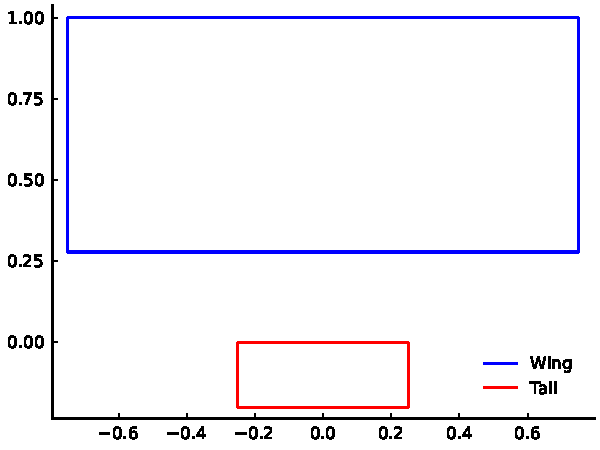
\includegraphics{../graphics/length_design.pdf}
		\caption{\emph{This figure shows design of an airframe with a length from wing to tail of 1.0 m.}}
		\label{fig:length_design}
	\end{figure}
	
	\subsection{Altered Wing Taper}
	The wing taper ratio of an airframe is found using equation \ref{eqn:taper-ratio}.
	
	\begin{equation}
		Taper\ Ratio = \frac{tip\ chord\ length}{base\ chord\ length}
		\label{eqn:taper-ratio}
	\end{equation}
	
	When evaluating an airframe that has a wing taper ratio that is less than 1.0 (I used 0.5), it was found that the velocity needed to calculate the necessary lift was 13.215339717762241 m/s. While this is close to the velocity needed for the optimized airframe, it is still larger; therefore, it is not as optimal. This shows that as the wing taper ratio is decreased, the velocity needed to lift 0.5 kilograms increases, making it sub-optimal. You can also see that an airframe with a wing taper ratio of 1.0 has a lift coefficient distribution that is closer to the optimal elliptical distribution than the airframe with a wing taper ratio of 0.5 (see figures \ref{fig:cl_dist} and \ref{fig:cl_dist_compare}).\\
	
	\begin{figure}[H]
		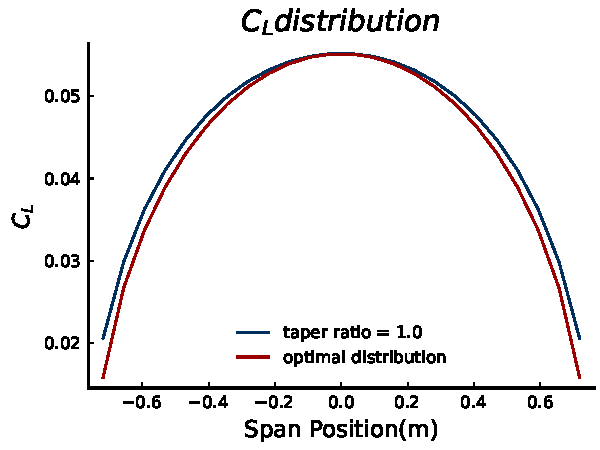
\includegraphics{../graphics/cl_dist.pdf}
		\caption{\emph{This figure shows the lift coefficient distribution for a taper ratio of 1.0 vs. the optimal elliptical distribution.}}
		\label{fig:cl_dist}
	\end{figure}
	\begin{figure}[H]
		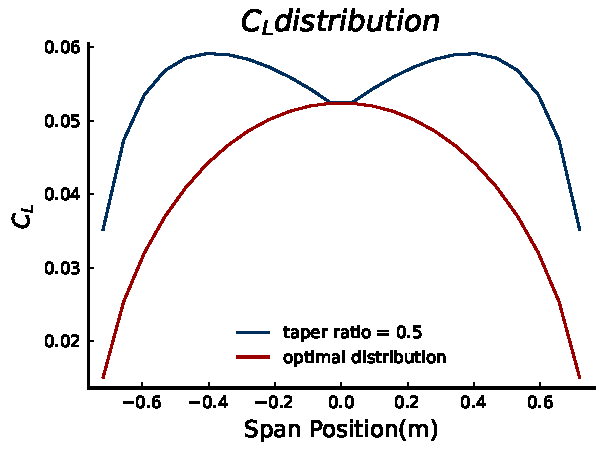
\includegraphics{../graphics/cl_dist_compare.pdf}
		\caption{\emph{This figure shows the lift coefficient distribution for a taper ratio of 0.5 vs. the optimal elliptical distribution.}}
		\label{fig:cl_dist_compare}
	\end{figure}
	
	Plots showing the lift coefficients and drag coefficients vs. angle of attack for these 2 designs are given (see figures \ref{fig:taper_cl} and \ref{fig:taper_cd}).
	
	\begin{figure}[H]
		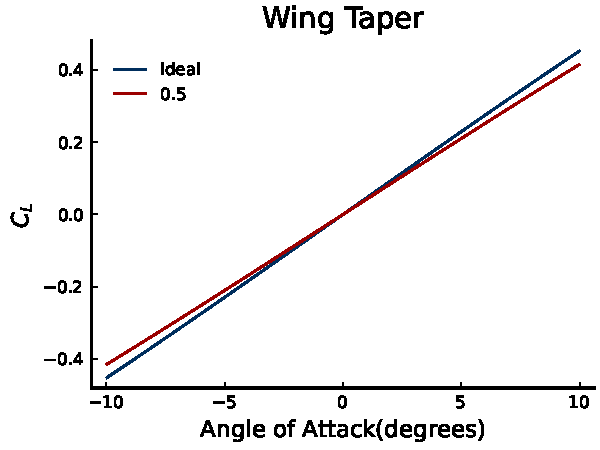
\includegraphics{../graphics/taper_cl.pdf}
		\caption{\emph{This figure shows the lift coefficients for varying angles of attack for the 2 designs evaluated using different wing tip tapers}}
		\label{fig:taper_cl}
	\end{figure}
	\begin{figure}[H]
		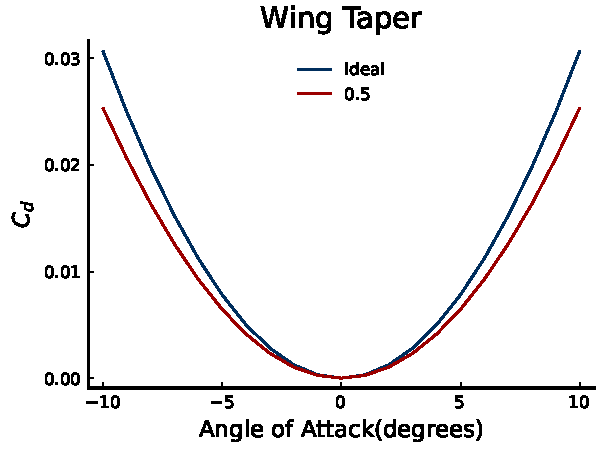
\includegraphics{../graphics/taper_cd.pdf}
		\caption{\emph{This figure shows the drag coefficients for varying angles of attack for the 2 designs evaluated using different wing tip tapers}}
		\label{fig:taper_cd}
	\end{figure}
	
	The design of an airframe with a wing taper ratio of 0.5 is shown in figure \ref{fig:taper_design}.
	
	\begin{figure}[H]
		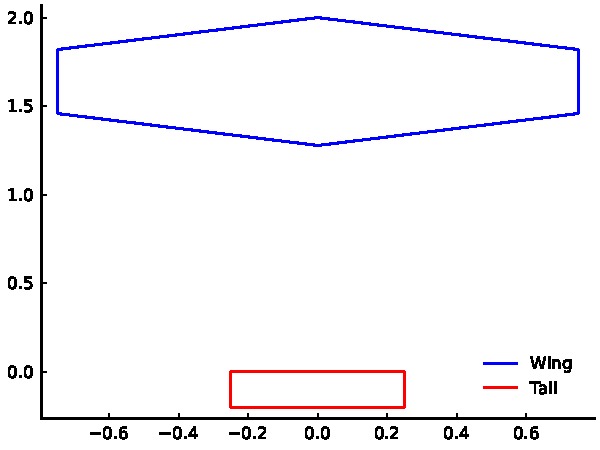
\includegraphics{../graphics/taper_design.pdf}
		\caption{\emph{This figure shows the design of an airframe with a wing taper ratio of 0.5.}}
		\label{fig:taper_design}
	\end{figure}

	\section{Conclusion}
	Here are some key findings from all of my research done on airframe design:
	 \begin{itemize}
	 	\item Higher Reynolds numbers cause the lift curves to become more steep and the drag and moment curves to become more leveled out for an airfoil.
	 	\item As the thickness of the airfoil increases, the airfoil's ratio of lift to drag curve becomes more shallow. As the camber of the airfoil increases, the lift to drag ratio becomes higher and the whole curve is shifted upwards. 
	 	\item The larger the tail of an airframe, the more stable it will be. However, bigger does not always mean better in this case.
	 	\item The Vortex Lattice Method for evaluating airframes in only accurate for small angles of attack, but is very powerful when used.
	 	\item The airframe that will generate the most lift will have a large wingspan and a large mean chord length. However, when designing an airframe, a lot more factors go into the design other than how much lift it produces.
	 	\item The most efficient airframe is one that has a wing taper ratio of 1.0, as it produces a lift coefficient distribution that is elliptical.
	 \end{itemize}

	\newpage
	
	\section{Appendix}
	
	\begin{itemize}
		\item Irrotational flow: a flow in which each element of the moving fluid undergoes no net rotation with respect to a chosen coordinate axes from one instant to other
		\item Inviscid: having no or negligible viscosity
		\item Chord: a straight line from the leading edge to the trailing edge (see figure \ref{fig:airfoil-diagram})
		\item Airfoil camber: the asymmetry between the two acting surfaces of an airfoil, with the top surface of a wing commonly being more convex. An airfoil that is not cambered is called a symmetric airfoil (see figure \ref{fig:airfoil-diagram})
		\item Airfoil thickness: the greatest distance between the upper and the lower surfaces of an airfoil (see figure \ref{fig:airfoil-diagram})
		
		\begin{figure}[H]
			\centering
			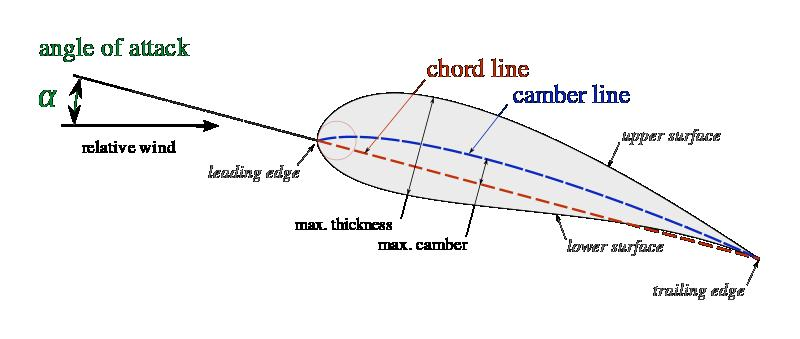
\includegraphics[scale=0.4]{../graphics/airfoil-diagram.jpg}
			\caption{\emph{airfoil diagram showing angle of attack, airfoil camber, thickness, and chord}}
			\label{fig:airfoil-diagram}
		\end{figure}
		
		\item Potential flow: an idealized model of fluid flow that occurs in the case of incompressible, inviscid, and irrotational flow
		\item Freestream: the air far upstream of an aerodynamic body, that is, before the body has a chance to deflect, slow down or compress the air
		\item Angle of attack: the angle at which the chord of an aircraft's wing meets the relative wind
		\item Drag coefficient: equal to the drag D divided by density r times half the velocity V squared times the reference area A. It expresses the ratio of the drag force to the force produced by the dynamic pressure times the area (see equation \ref{eqn:drag})
		
		\begin{equation}
			\centering
			\label{eqn:drag}
			c_d = \frac{2D}{\rho{V^2}S}
		\end{equation}
		
		\item Lift coefficient: relates the lift generated by a lifting body to the fluid density around the body, the fluid velocity and an associated reference area (see equation \ref{eqn:lift})
		
		\begin{equation}
			\centering
			\label{eqn:lift}
			c_\ell = \frac{2L}{\rho{V^2}S}
		\end{equation}
		
		\item Moment coefficient: pertains to the moment specifically due to the aerodynamics force (see equation \ref{eqn:moment})
		
		\begin{equation}
			\centering
			\label{eqn:moment}
			c_m = \frac{2M}{\rho{V^2}S}
		\end{equation}
		
		\item Stall: a sudden reduction in the lift generated by an aerofoil when the critical angle of attack is reached or exceeded	
		\item Airfoil polar: represent the aerodynamic characteristics of an airfoil (figure \ref{fig:aoa-coefficients} is an example of an airfoil polar)
		\item Reynold's number: helps predict flow patterns in different fluid flow situations. At low Reynolds numbers, flows tend to be dominated by laminar (sheet-like) flow, while at high Reynolds numbers flows tend to be turbulent. Equation \ref{eqn:velocity} calculates Reynold's number using \(\rho\)(density), u(flow speed), L(characteristic linear dimension), and \(\mu\)(dynamic viscosity of fluid)
		
		\begin{equation}
			\centering
			\label{eqn:velocity}
			R_e = \frac{\rho{uL}}{\mu}
		\end{equation}
		
		\item Mach number: ratio of the speed of a body to the speed of sound in the surrounding medium
		\item Lift curve slope: measure of how rapidly the wing generates lift with change in AOA (see figure \ref{fig:lift-curve-slope})
		
		\begin{figure}[H]
			\centering
			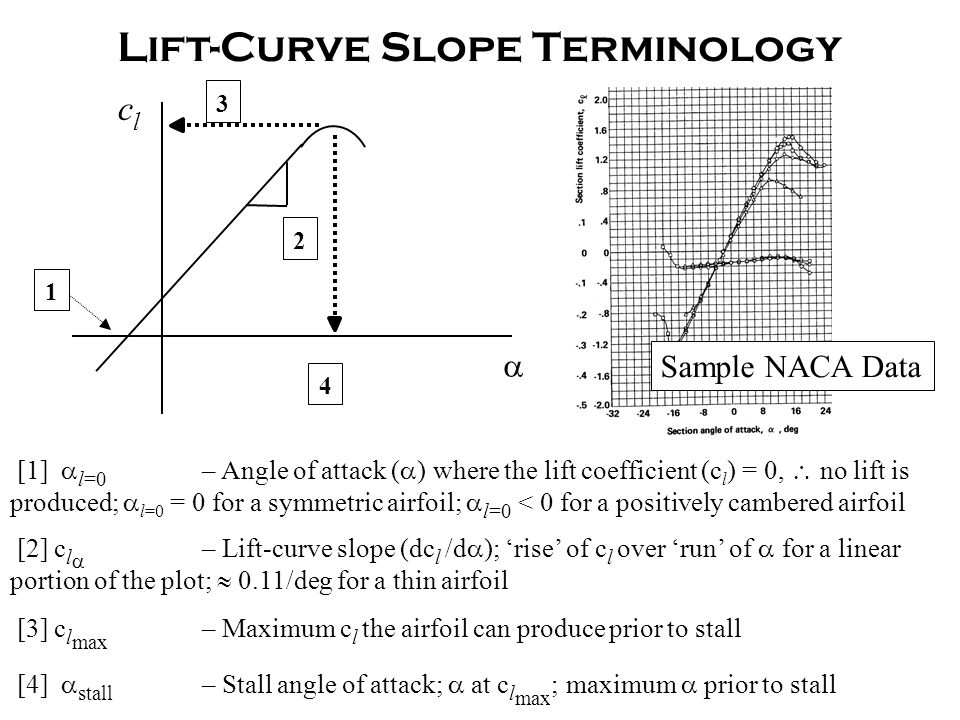
\includegraphics[scale=0.4]{../graphics/lift-curve-slope.jpg}
			\caption{\emph{This diagram shows the major characteristics of a lift curve}}
			\label{fig:lift-curve-slope}
		\end{figure}
	
		\item Sweep: the angle at which the wing is translated backwards (or occasionally forwards) relative to the root chord of the wing (see figure \ref{fig:sweep})
		
		\begin{figure}[H]
			\centering
			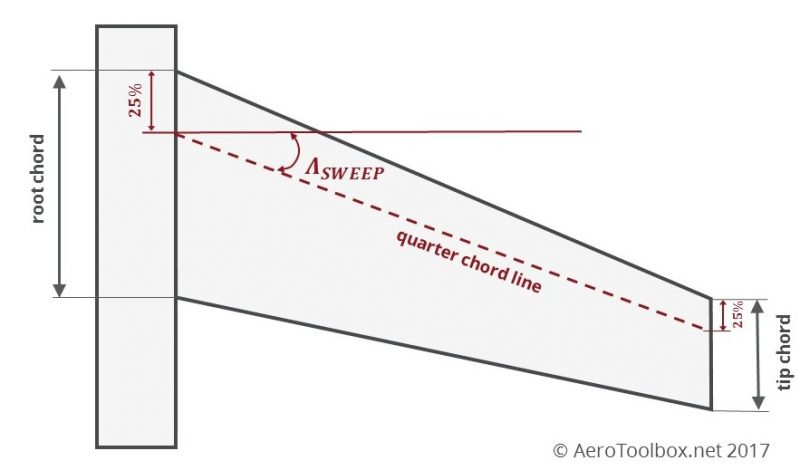
\includegraphics[scale=0.4]{../graphics/sweep.jpg}
			\caption{\emph{This diagram shows what sweep is on an airframe.}}
			\label{fig:sweep}
		\end{figure}
		
		\item Aspect Ratio: aspect ratio of a wing is the ratio of its span to its mean chord. It is equal to the square of the wingspan divided by the wing area. Thus, a long, narrow wing has a high aspect ratio, whereas a short, wide wing has a low aspect ratio (see equation \ref{eqn:aspect-ratio-wiki})
		
		\begin{equation}
			AR = \frac{b}{c} = \frac{b^2}{S_{ref}}
			\label{eqn:aspect-ratio-wiki}
		\end{equation}
		
		\item Wake Vortex/Tip Vortex: a lifting wing has higher pressure on the bottom surface as compared to the top, and so fluid will circulate around the tips (see figure \ref{fig:downwash-wakevortex})
		\item Downwash: can be viewed more fundamentally as a consequence of Newton’s third law. If a body is producing lift, colloquially we might say that means that the air is pushing the body up. Thus, by Newton’s third law, the body must be pushing the air downward. Thus, any three-dimensional lifting body will leave behind a wake of downward moving air (see figure \ref{fig:downwash-wakevortex})
		
		\begin{figure}
			\centering
			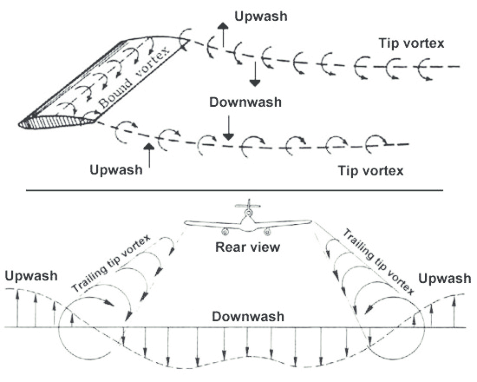
\includegraphics[scale=0.4]{../graphics/downwash-wakevortex.png}
			\caption{\emph{This diagram shows how downwash and wake vortexes are formed.}}
			\label{fig:downwash-wakevortex}
		\end{figure}
		
		\item Induced Drag/Vortex Drag: major consequence of this downwash, is that energy is left behind in the wake. Or in other words, the wing produces drag
		\item Inviscid Span Efficiency:  the inviscid span efficiency could be considered a measure of how close the lift distribution is to elliptic. All planar distributions will have \(e_{inv} <= 1\). A nonplanar lift distribution (e.g., adding winglets) can increase the inviscid span efficiency above 1 (see equation \ref{eqn:efficiency-wiki})
		
		\begin{equation}
			e_{inv} = \frac{C_L^2}{\pi{ARC_D}}
			\label{eqn:efficiency-wiki}
		\end{equation}
		
		\item Vortex Filament: an arbitrary vortex line segment
		\item Vortex Lattice Method: an extension of thin airfoil theory into three dimensions
		\item Tail Volume Ratio: relates the shape of the tail to the wing 
		\subitem Vertical Tail Volume Ratio: 
		
		\begin{equation}
			V_v = \frac{l_vS_v}{Sb}
			\label{eqn:vtail-ratio-wiki}
		\end{equation}
		
		\subitem Horizontal Tail Volume Ratio:
		
		\begin{equation}
			V_h = \frac{l_tS_t}{SC_{ma}}
			\label{eqn:htail-ratio-wiki}
		\end{equation}
		
		\item Stability Derivatives: measures of how particular forces and moments on an aircraft change as other parameters related to stability change
		
		\item Engineering Design - an iterative process that engineers follow to
		develop a product that accomplishes a given task (see figure \ref{fig:design-process}).
		
		\begin{figure}[H]
			\centering
			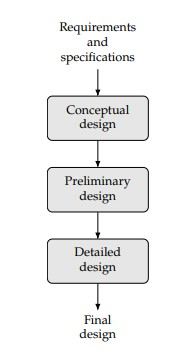
\includegraphics[scale=0.75]{../graphics/design_process}
			\caption{\emph{This figure shows the steps of the engineering design process.}}
			\label{fig:design-process}
		\end{figure}
		
		\item Design Optimization Process - s a tool that can replace an iterative design
		process to accelerate the design cycle and obtain better results (see figure \ref{fig:optimization}).
		
		\begin{figure}[H]
			\centering
			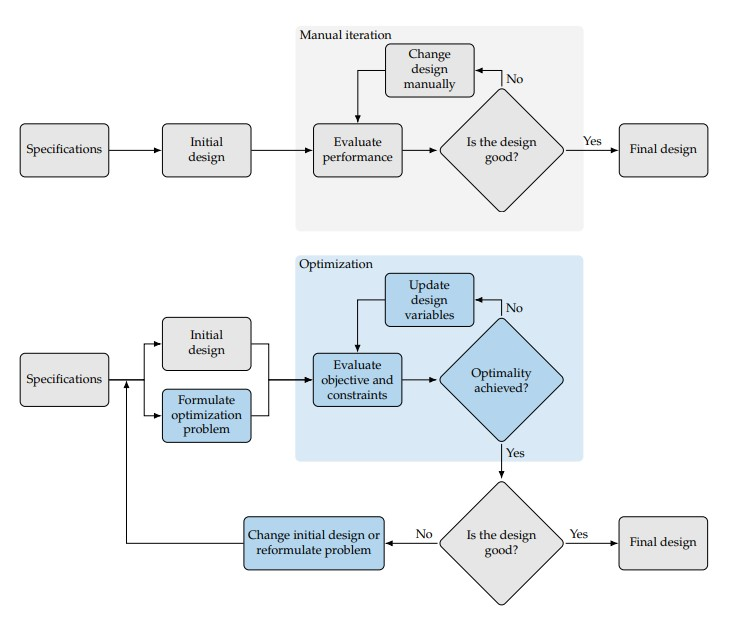
\includegraphics[scale=0.5]{../graphics/optimization_process}
			\caption{\emph{This figure shows the steps of the engineering design optimization process.}}
			\label{fig:optimization}
		\end{figure}
		
		\item Objective Function - the design optimization process requires the designer to translate their intent to a mathematical statement that can then be solved by an optimization algorithm
		\item Design Variables - the variables that describe the system, must not depend on each other or any other parameter
		
	\end{itemize}
	
\end{document}